\chapter{Исследовательский раздел}
\label{cha:research}

В данном разделе привидены и проанализированы примеры работы программы редакционного расстояния.

\section{Примеры работы}

На рисунках 4.1, 4.2, 4.3, 4.4 показана работа программы с различными входными данными.

\begin{figure}[H]
\centering
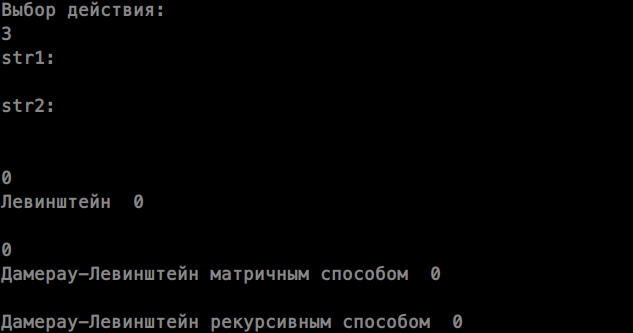
\includegraphics[scale=0.75]{./pict/5rr.png}
\caption{Пустое слово}
\end{figure}
\begin{figure}[H]
\centering
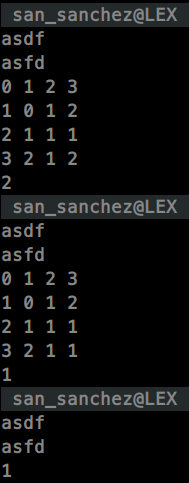
\includegraphics[scale=0.75]{./pict/work_transpos.png}
\caption{Транспозиция}
\end{figure}
\begin{figure}[H]
\centering
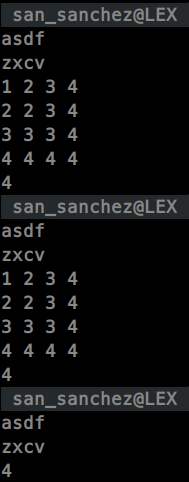
\includegraphics[scale=0.75]{./pict/work_diff_words.png}
\caption{Разные слова}
\end{figure}
\begin{figure}[H]
\centering
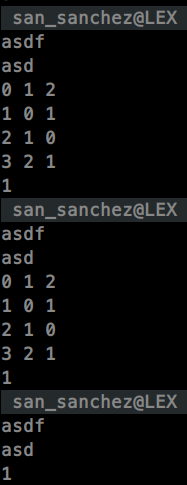
\includegraphics[scale=0.75]{./pict/work_without_symb.png}
\caption{Пропущена одна буква}
\end{figure}


\section{Эксперименты по замеру времени}
Чтобы подтвердить вывод об оценке сложности алгоритмов поиска редакционного расстояния, проведём эксперименты по замеру времени и построим графики зависимости времени выполнения данных алгоритмов от длины обрабатываемых слов.

\subsection{Эксперимент 1}
На рисунке 4.5 приведён график сравнения алгоритма Вагнера-Фишера и матричного алгоритма Дамерау-Левенштейна. Для этого эксперимента было сгенерировано 100 пар полностью не совпадающих строк с диапазоном длин от 10 до 1000. Как видно, законы изменения времени выполнения этих алгоритмов практически одинаковы и отличаются лишь на некоторый постоянный коэффициент.
\begin{figure}[H]
    \centering
    \begin{tikzpicture}
        \begin{axis}[
            width=0.8*\linewidth,
            xlabel={Длина слова},
            ylabel={Время (нс)},
            grid=major,
            legend pos=north west,
        ]

        \addplot[color=red]
            table[x=len,y=time,col sep=comma]{./data/wagner-fischer-1.csv};
        \addplot[color=blue]
            table[x=len,y=time,col sep=comma]{./data/damerau-levenshtein-1.csv};

        \legend{Вагнера-Фишера, Дамерау-Левенштейна}

        \end{axis}
    \end{tikzpicture}
    \caption{График сравнения алгоритма Вагнера-Фишера и матричного алгоритма Дамерау-Левенштейна}
\end{figure}

\subsection{Эксперимент 2}
На рисунке 4.6 приведён график сравнения рекурсивного и матричного алгоритмов нахождения расстояния Дамерау-Левенштейна. Для этого эксперимента было сгенерировано 10 пар полностью различных слов с диапазоном длин от 1 до 10. Количество времени, необходимого для выполнения рекурсивного алгоритма, растёт экспоненциально, в то время как сложность матричного алгоритма имеет квадратичный рост, что наглядно изображено на рисунке 4.5.
\begin{figure}[H]
    \centering
    \begin{tikzpicture}
        \begin{axis}[
            width=0.8*\linewidth,
            xlabel={Длина слов},
            ylabel={Время (нс)},
            grid=major,
            legend pos=north west,
        ]

        \addplot[color=red]
            table[x=len,y=time,col sep=comma]{./data/damerau-levenshtein-rec-2.csv};
        \addplot[color=blue]
            table[x=len,y=time,col sep=comma]{./data/damerau-levenshtein-2.csv};

        \legend{рекурсивный, матричный}

        \end{axis}
    \end{tikzpicture}
    \caption{График времени работы реализаций рекурсивного и матричного алгоритмов Дамерау-Левенштейна}
\end{figure}

\pagebreak

\section{Вывод}

Как итог, была подтверждена корректная работоспособность реализованной программы нахождения расстояний Левенштейна и Дамерау-Левенштейна и доказаны тезисы, составленные в результате анализа этих алгоритмов.

